\clearpage
\section{V1: Fixed-Identity Geometry Study}\label{app:v1}
This appendix preserves the earlier algorithm and its evidence. Every occurrence of ``Ours'' embedded in a retained V1 figure denotes V1 only; the current method is identified as \ours{} in the new main result and outdoor appendices. The versions do not share an evaluation protocol.

\subsection{Depth-conditioned support, refutation, and deletion}
For source point $p$ assigned to object $o$, V1 projects into frames with an assigned observation. It requires positive camera depth $z>0.2$\,m and a finite positive measured depth $D$ satisfying $|z-D|\leq0.05\,\mathrm m+0.01D$. An eligible projection supports $o$ inside its eroded mask union, or refutes $o$ inside another known mask outside the dilated union. The erosion/dilation radius is two pixels. Unknown pixels, occlusions, and uncertain boundaries abstain; overlapping masks contribute at most one vote per point/frame. With support $S_o(p)$ and refutation $R_o(p)$ accumulated over eligible frames, V1 deletes exactly when
\begin{equation}
R_o(p)\geq1\quad\land\quad R_o(p)\geq2S_o(p).
\label{eq:v1-rule}
\end{equation}
For nonzero evidence this is equivalent to support share $S/(S+R)\leq1/3$; zero-evidence points remain. It cannot append surfaces, create objects, split mergers, or revise identity. Statistical outlier removal (SOR)~\cite{sor} uses each object's mean 20-neighbor distance with a mean-plus-two-standard-deviations cutoff. These are separate point-selection mechanisms.

\subsection{Configuration selection}
Replica~\cite{replica} office\_0/office\_1 and SceneNN 014/015 were exposed development data. The pilot primary required three refutations. Before processing the four new SceneNN scenes, the existing one-refutation arm was selected empirically: its dataset-mean gains were +2.018 and +1.034 points, versus +2.002 and +0.656 for three refutations. Only the minimum count changed; the depth gate, boundaries, and refutation/support ratio remained fixed. This did not make the original two-point-per-dataset pilot requirement pass. V1 also remained below SOR in the subsequent four-scene mean. No configuration was selected after those new-scene scores.

\begin{center}\small
\begin{tabular}{lrrrrr}
\toprule
Scene & Baseline & SOR & Three-frame & No depth (3) & V1 (1) \\
\midrule
office\_0 & 30.923 & 31.249 & 34.017 & 33.589 & 34.078 \\
office\_1 & 47.019 & 47.752 & 47.928 & 45.289 & 47.900 \\
SN 014 & 15.868 & 16.452 & 17.133 & 17.068 & 17.824 \\
SN 015 & 14.408 & 14.669 & 14.454 & 14.422 & 14.519 \\
\bottomrule
\end{tabular}

\captionof{table}{V1 development PQ, kept separate from both SceneNN new-scene and current KITTI-360 results. ``No depth (3)'' uses three refutations, unlike the one-refutation no-depth control in the SceneNN main table.}
\end{center}

\begin{minipage}[t]{.49\textwidth}\vspace{0pt}\centering\small
\begin{tabular}{lrr}
\toprule
Contrast & $\Delta$ PQ & Wins/losses \\
\midrule
V1 -- baseline & +0.841 & 4/0 \\
V1 -- SOR & -0.050 & 3/1 \\
V1 -- no depth & +0.454 & 2/2 \\
V1 -- three-frame & +0.136 & 4/0 \\
V1 locked -- baseline & +1.095 & 4/0 \\
SOR locked -- baseline & -0.287 & 2/2 \\
\bottomrule
\end{tabular}

\captionof{table}{V1 paired contrasts on four SceneNN scenes. Locked assignment is a diagnostic, not the primary metric.}
\end{minipage}\hfill
\begin{minipage}[t]{.48\textwidth}\vspace{0pt}\centering\small
\begin{tabular}{lrrrr}
\toprule
Scene & Objects & Points & Evidence (s) & Job (s) \\
\midrule
052 & 89 & 48,231 & 0.286 & 1.583 \\
054 & 121 & 70,796 & 0.458 & 1.949 \\
057 & 31 & 38,377 & 0.262 & 1.236 \\
061 & 12 & 60,913 & 0.391 & 1.836 \\
\bottomrule
\end{tabular}

\captionof{table}{V1 archived CPU timers and map scale. Evidence jointly times gated and ungated voting; job includes loading, SOR, cleanup variants and exports. Neither is isolated V1 latency or current-method speed.}
\end{minipage}

\subsection{Matched-set and assignment interpretation}
V1's 66 SceneNN matches are unchanged. At GT 136313 in scene 057, V1 gives IoU 0.496947 while SOR reaches 0.535340. V1 removes 92 source points and SOR removes 97: deletion count alone does not explain the ranking. Of 410 excess baseline reference voxels, 304 have owners with support but no refutation. Under locked baseline source ownership, V1 instead reaches IoU 0.501247; ordinary reassignment adds five correct and 17 excess voxels. Nearest-source reassignment therefore changes the measured effect of point deletion.


\clearpage
\section{V1 Architecture and Visibility Evidence}\label{app:v1-architecture}
The diagram below preserves the complete fixed-identity architecture and its evidence flow. It complements the current authorization architecture in Figure~\ref{fig:architecture}; the two diagrams describe different update operations.
\begin{center}
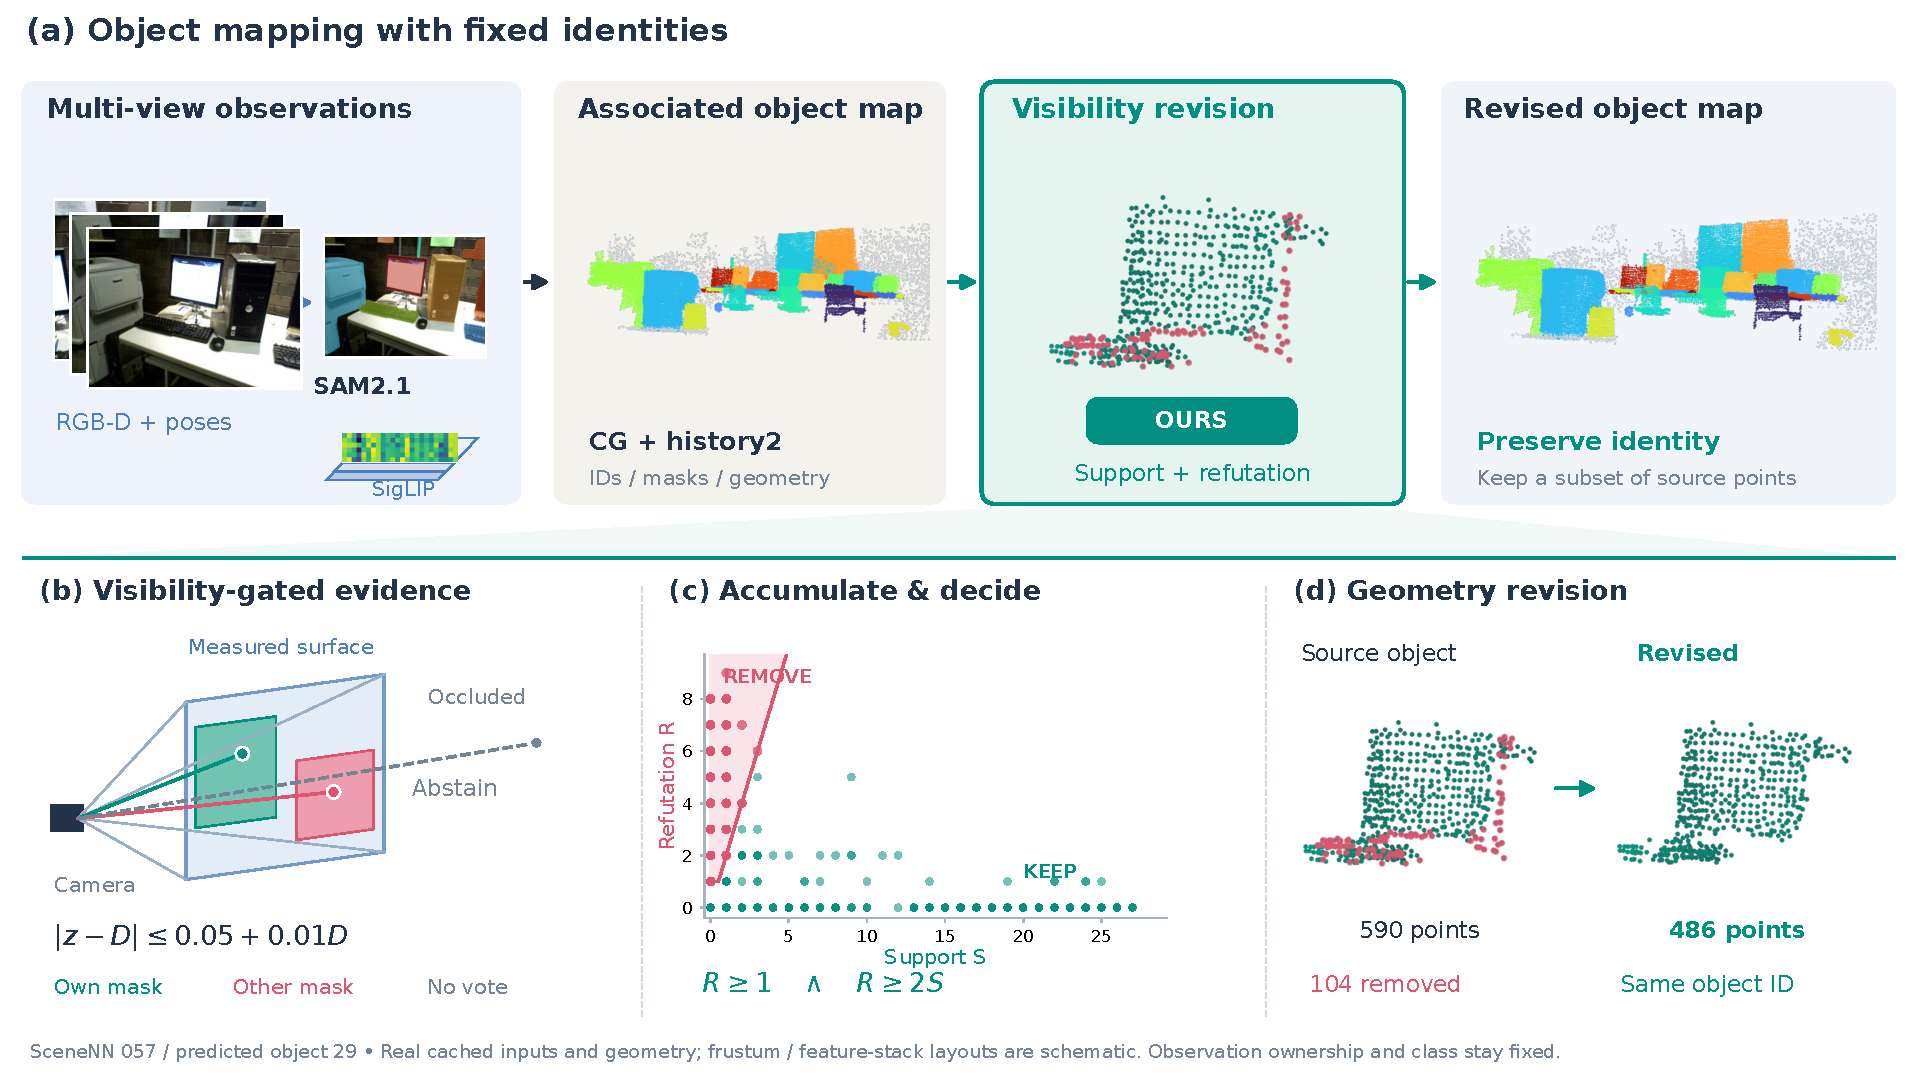
\includegraphics[width=\textwidth]{method_architecture.pdf}
\captionof{figure}{Retained V1 architecture with actual SceneNN observations, cached descriptors, source-point evidence, and revised object geometry. The embedded ``OURS'' block denotes V1. It retains a subset of existing source points while keeping identities, observation ownership, and semantic classes fixed. View frustums and the feature-stack layout are schematic.}
\label{fig:v1-architecture}
\end{center}
\subsection{Reading the two architectures together}
V1 asks whether a point already assigned to an object should remain in that object. Depth gating defines eligible observations; support and refutation determine deletion. It does not grant permission to change the historical identity of a point or append missing measurements.

The current method adds historical relabeling and measured-surface admission to the available updates. Figure~\ref{fig:architecture} shows this extension; the pose source remains fixed in both studies.

\clearpage
\section{Retained Indoor Image and Object Evidence}
\begin{center}
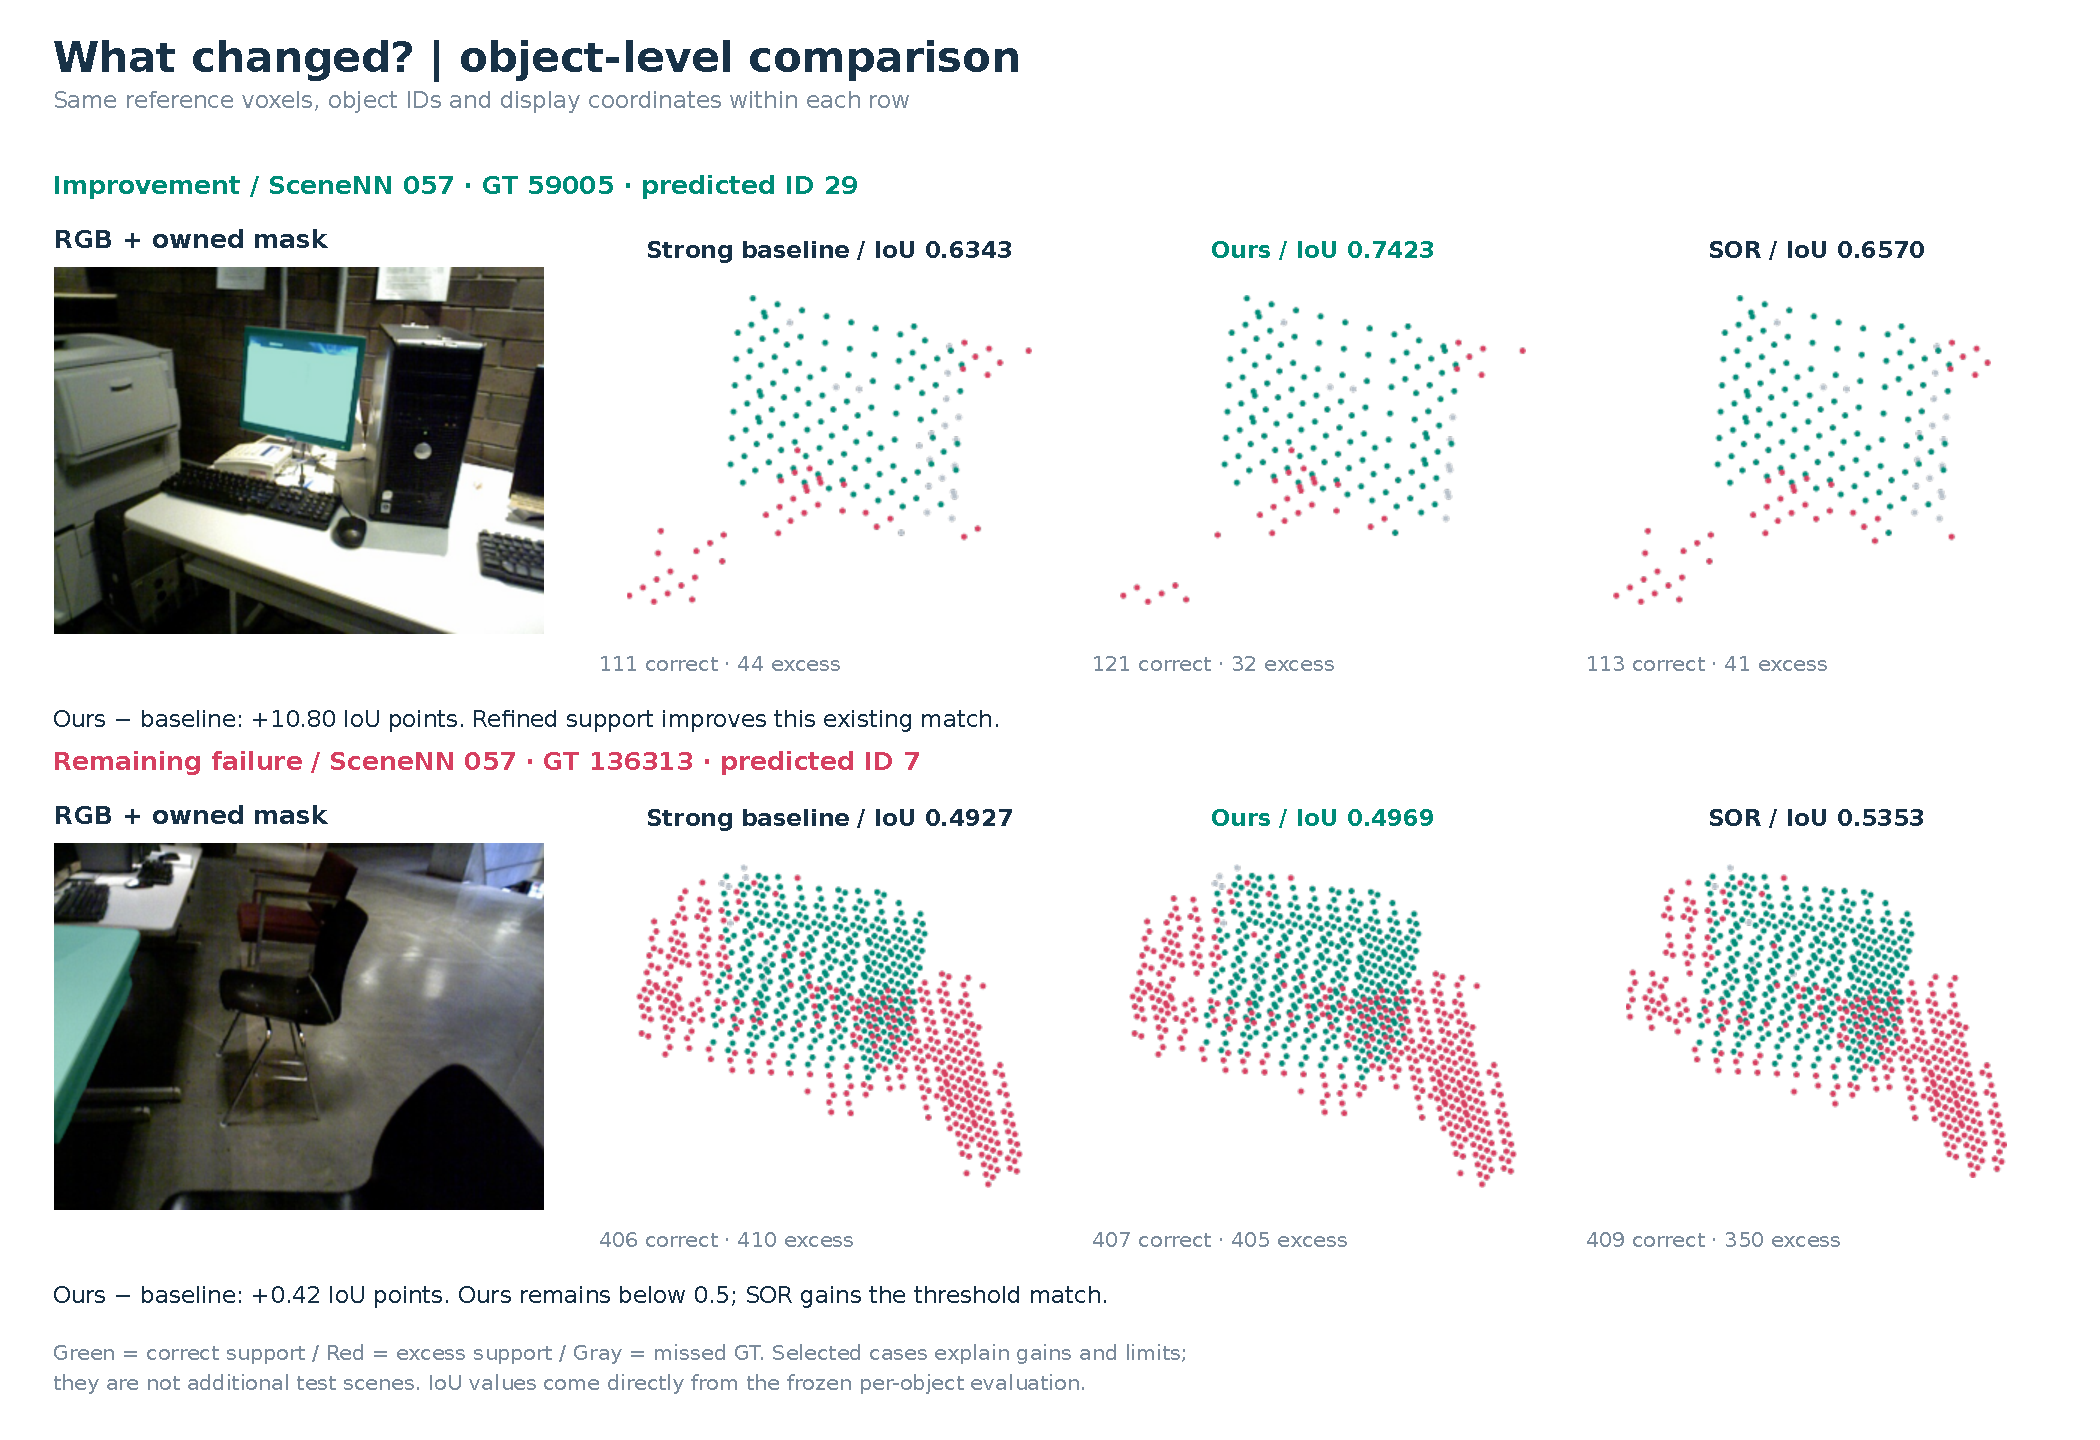
\includegraphics[width=\textwidth]{object_comparison_real.pdf}
\captionof{figure}{Actual SceneNN 057 observations and same-object geometry from V1. Embedded ``Ours'' labels mean V1. The monitor improves from IoU 0.6343 to 0.7423; the second object remains below 0.5 while SOR crosses it. These were post-evaluation explanatory selections, not random samples.}
\end{center}
These indoor images use supplied RGB-D poses and the SAM2.1/SigLIP branch. The following two pages retain each scene at full width so that RGB, masks, colored geometry, and predicted object boundaries can be inspected separately.

\clearpage
\section{SceneNN 057: Observations and V1 Map}
\begin{center}
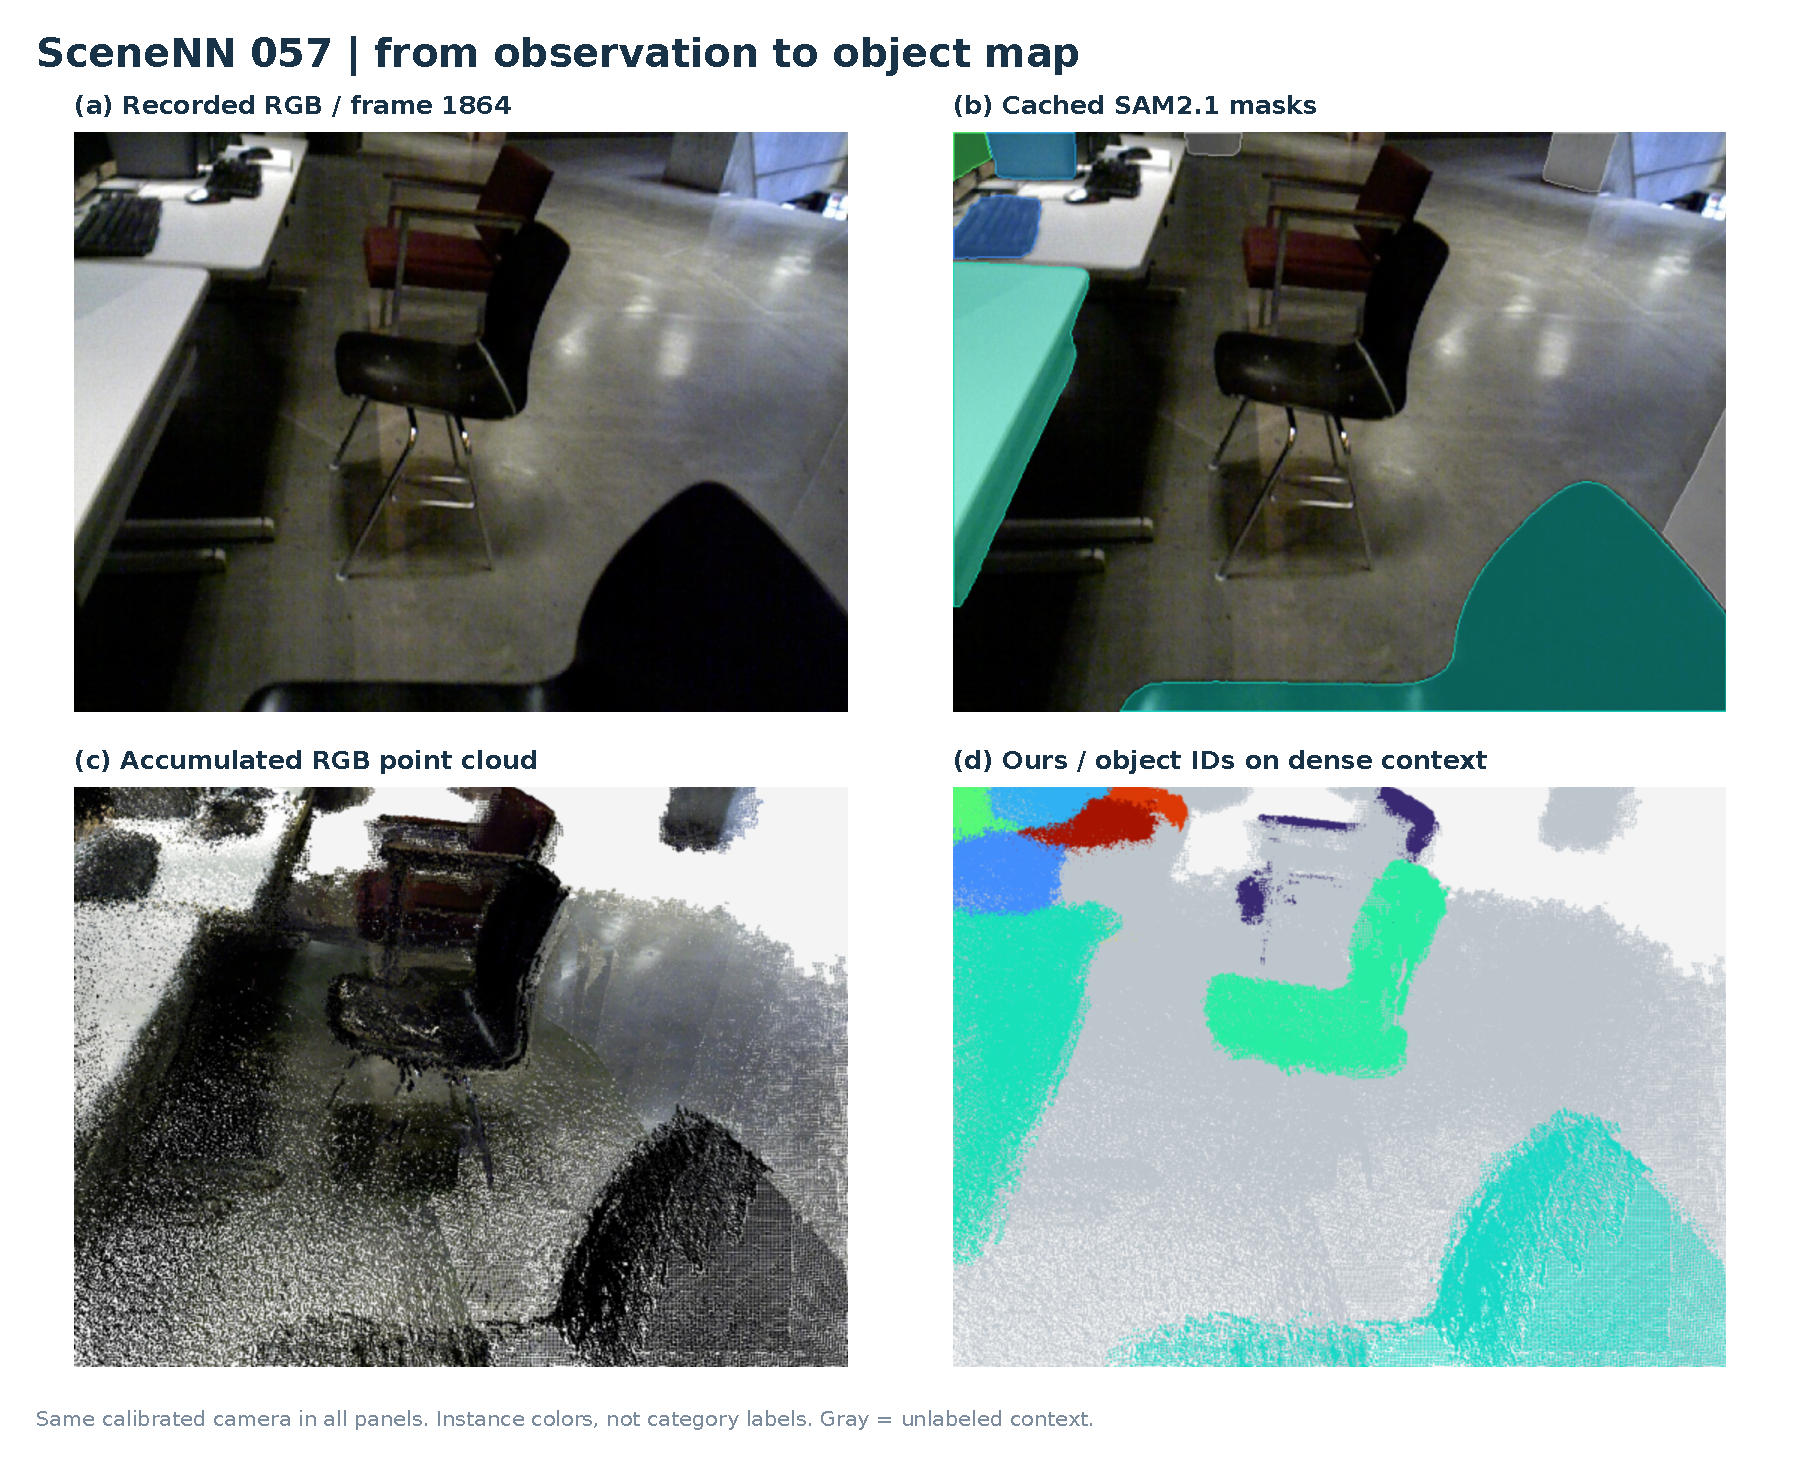
\includegraphics[width=.98\textwidth,height=.77\textheight,keepaspectratio]{dataset_scene_057.pdf}
\captionof{figure}{Actual RGB, cached SAM2.1 masks, accumulated colored geometry, and the V1 object map in one calibrated camera view. Embedded ``Ours'' means V1. The view was selected after evaluation to maximize support for predicted object 7. Point clouds use nearest-depth splats without hole completion. For dense display only, IDs transfer within 3\,cm; scoring uses 5\,cm on the observed-valid domain. Gray indicates unlabeled context. Colors encode predicted IDs, not GT classes.}
\end{center}

\clearpage
\section{SceneNN 061: A Second Evaluated V1 Scene}
\begin{center}
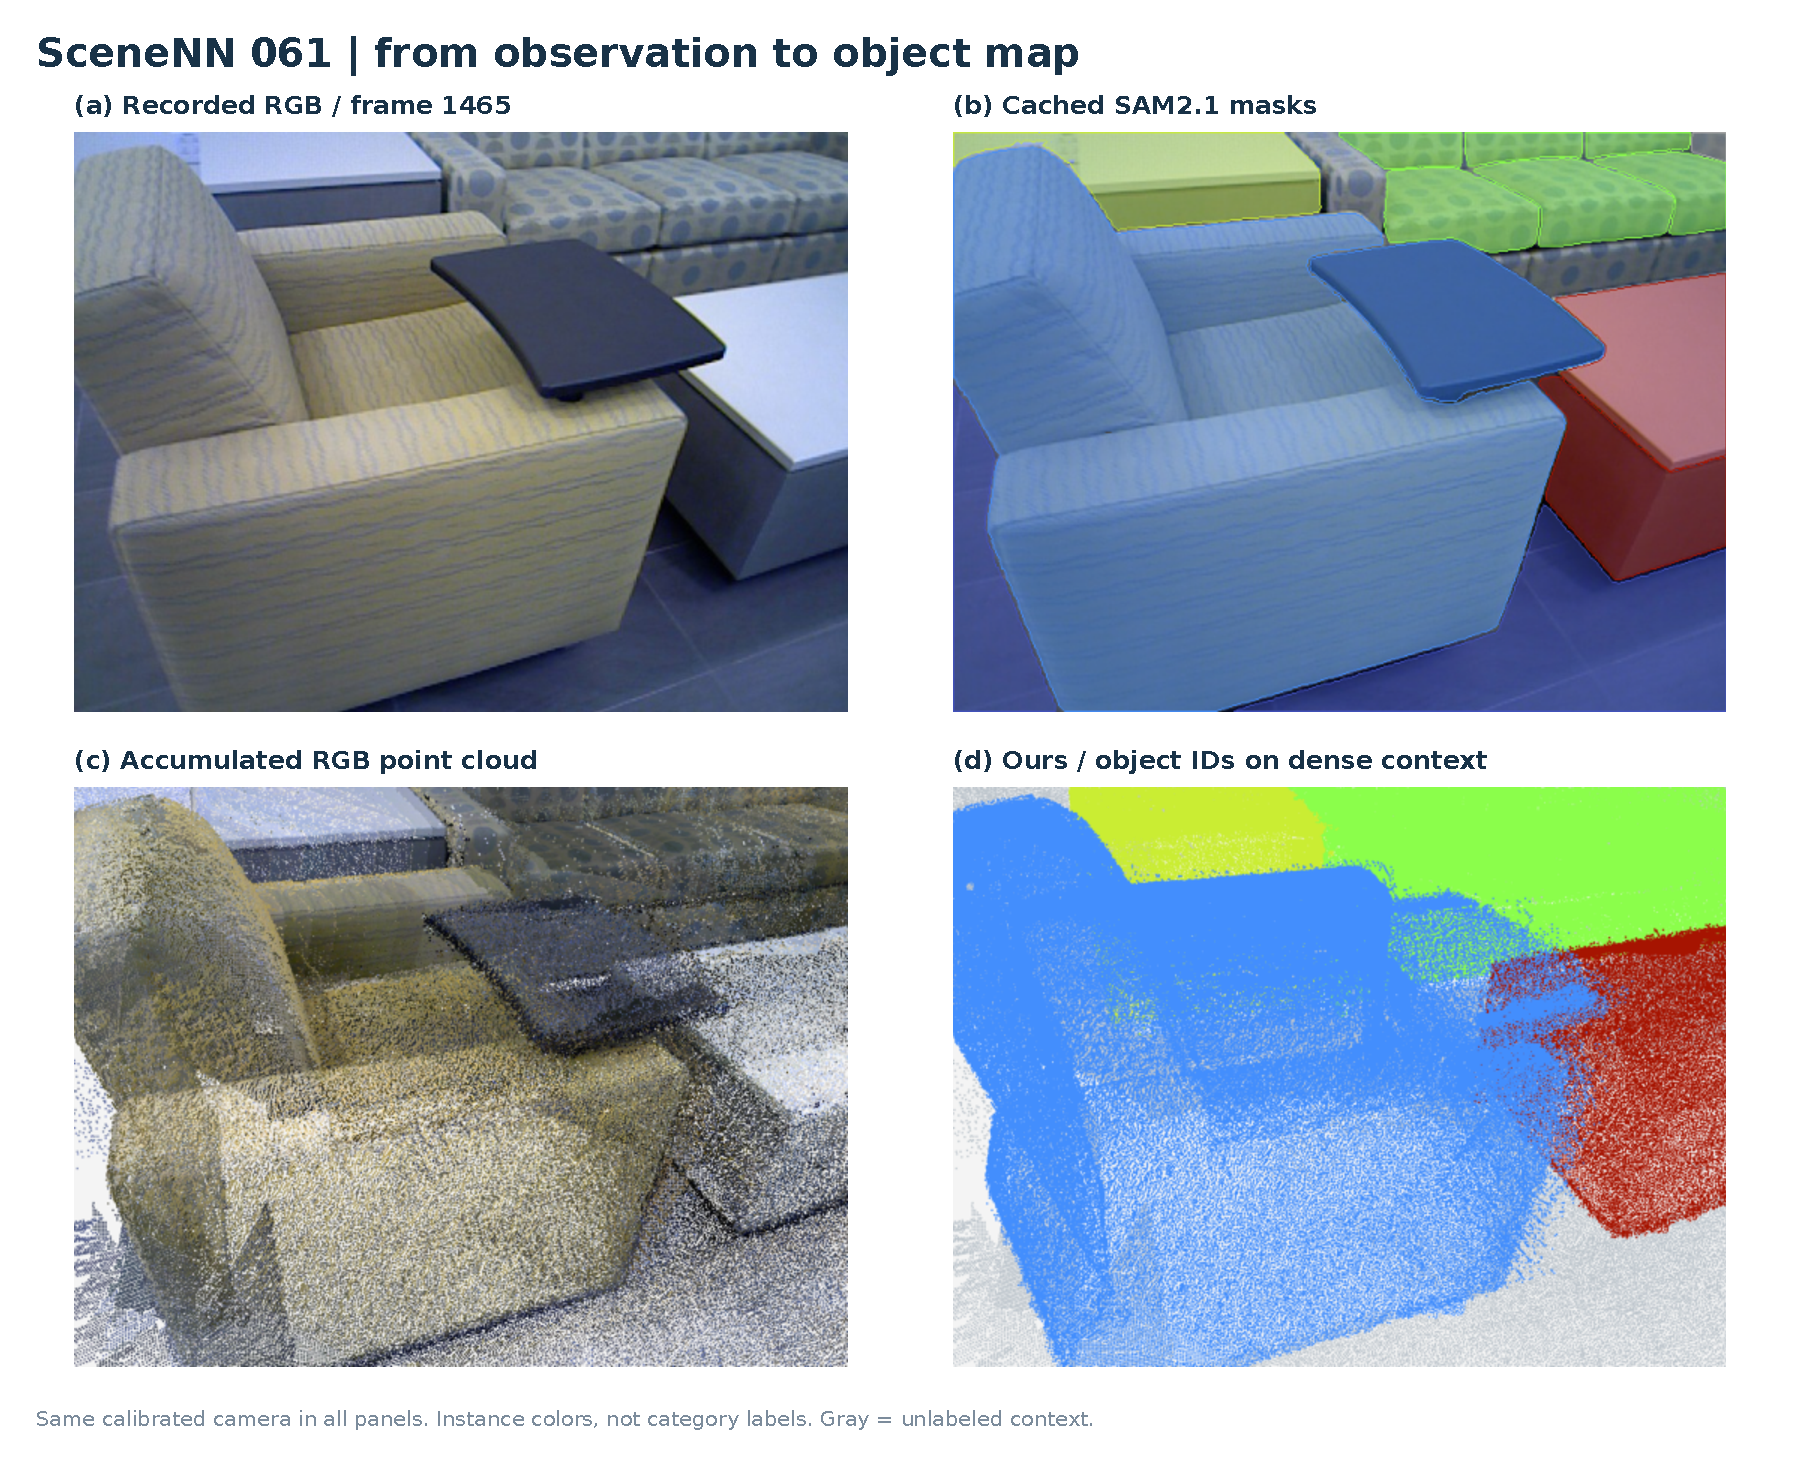
\includegraphics[width=.98\textwidth,height=.77\textheight,keepaspectratio]{dataset_scene_061.pdf}
\captionof{figure}{Real RGB and segmentation of the seating area, accumulated colored geometry, and V1 object IDs. Embedded ``Ours'' means V1. Display rules match the preceding page; the explanatory view maximizes cached support for predicted object 10. Accumulated geometry includes other viewpoints, so coverage need not match the single image. These are retained V1 results, not current-method cross-dataset runs.}
\end{center}
\clearpage
\section{V1 Development Gains and All-Object Changes}
The original development and new-scene plots are retained together with their exposure boundaries. ``Ours'' inside both plots denotes V1. The numerical tables and original predictions are unchanged.
\begin{center}
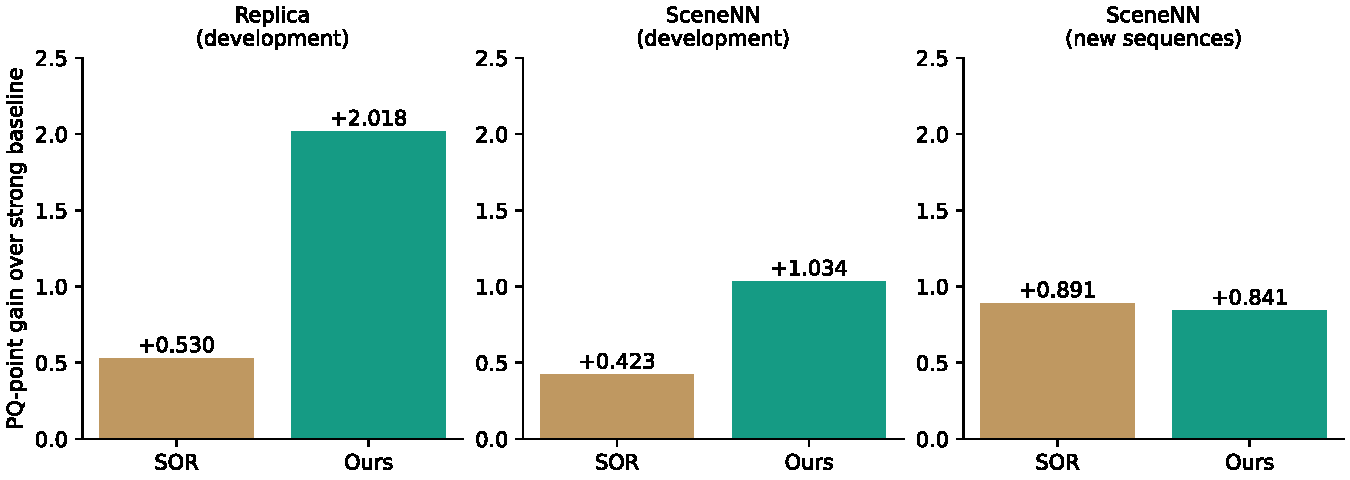
\includegraphics[width=\textwidth]{development_vs_unseen.pdf}
\captionof{figure}{PQ-point gains over the corresponding strong baseline, separated by dataset and development exposure. Replica office\_0/office\_1 and SceneNN 014/015 were exposed development scenes. Only the final group is the four new SceneNN sequences in the V1 main table. These gains do not describe current KITTI-360 authorization.}
\end{center}
\begin{center}
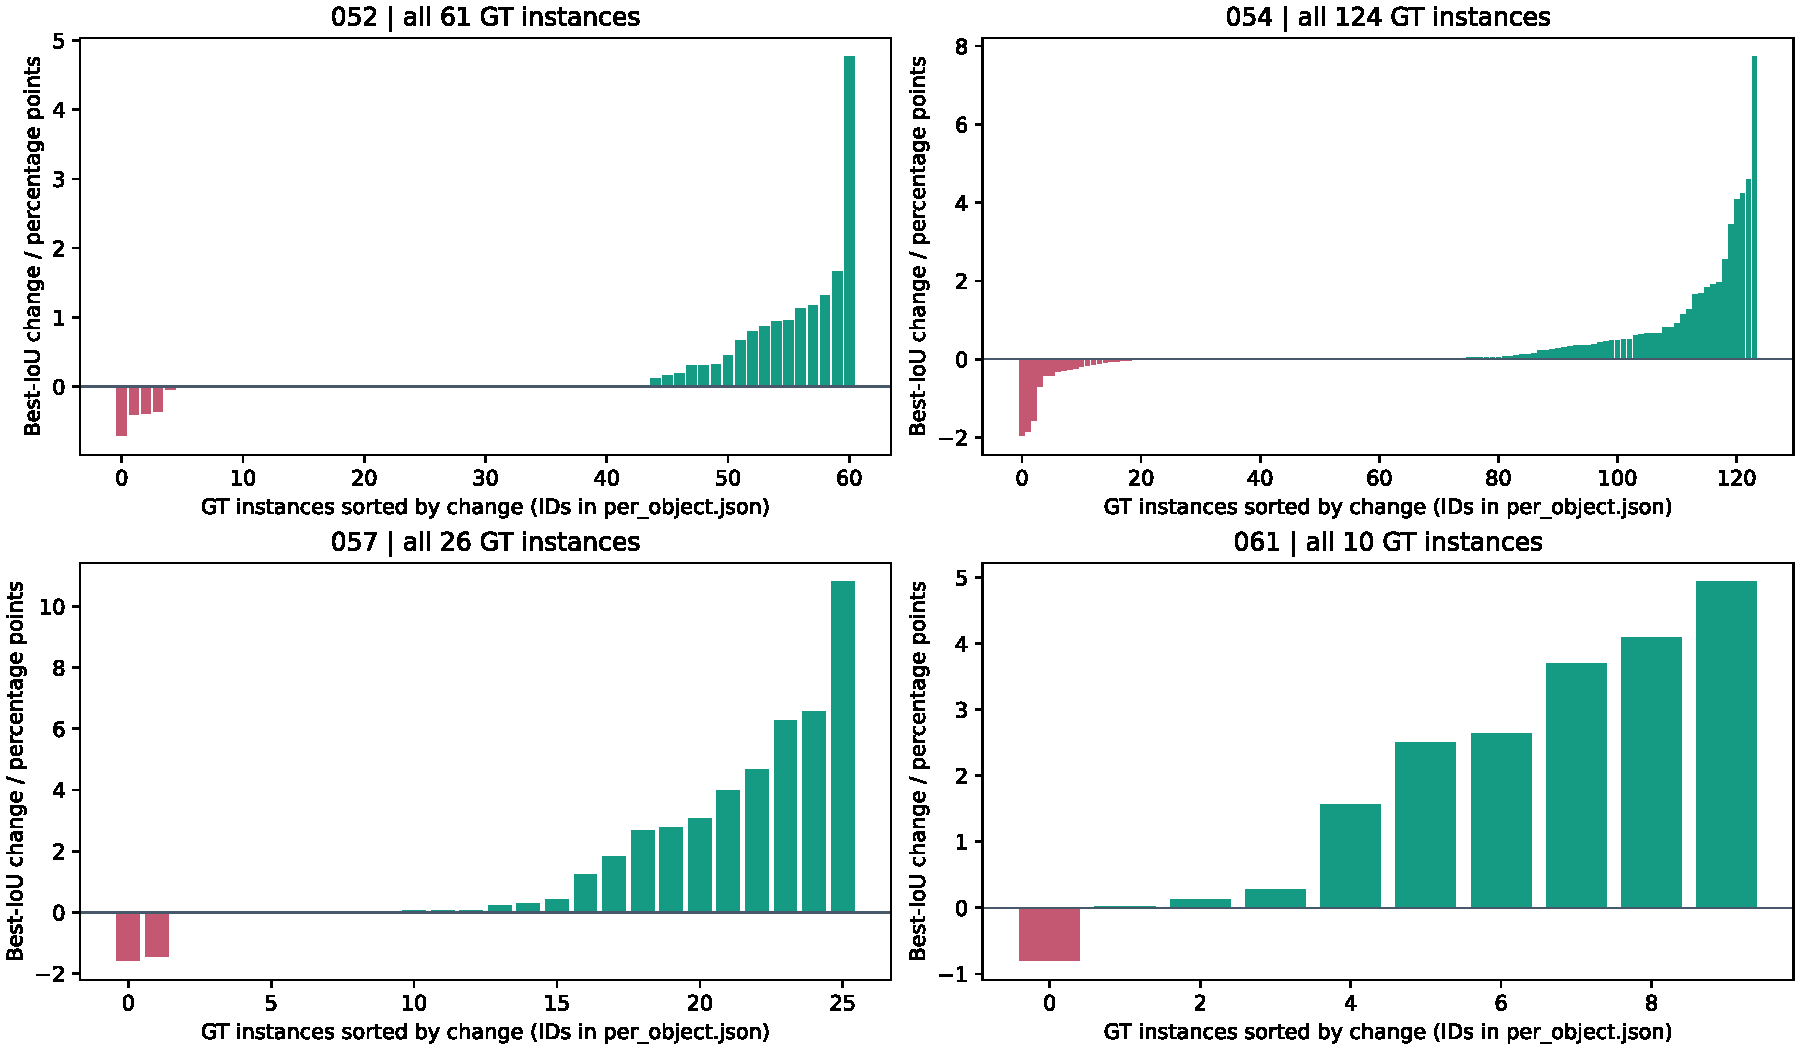
\includegraphics[width=\textwidth]{all_object_changes.pdf}
\captionof{figure}{Best-object IoU changes for all 221 GT instances in the four V1 SceneNN sequences. Objects are sorted by change within each scene; unchanged and regressed instances remain visible. There are 100 improvements, 27 declines, and 94 unchanged objects. Objects within a scene are not independent statistical trials.}
\end{center}

\clearpage
\section{V1 Evidence and Assignment Diagnostics}
These diagnostics explain why the V1 sequence-057 result trails SOR even though many individual geometries improve. They retain the original metric and the separately labeled locked-assignment diagnostic.
\begin{center}
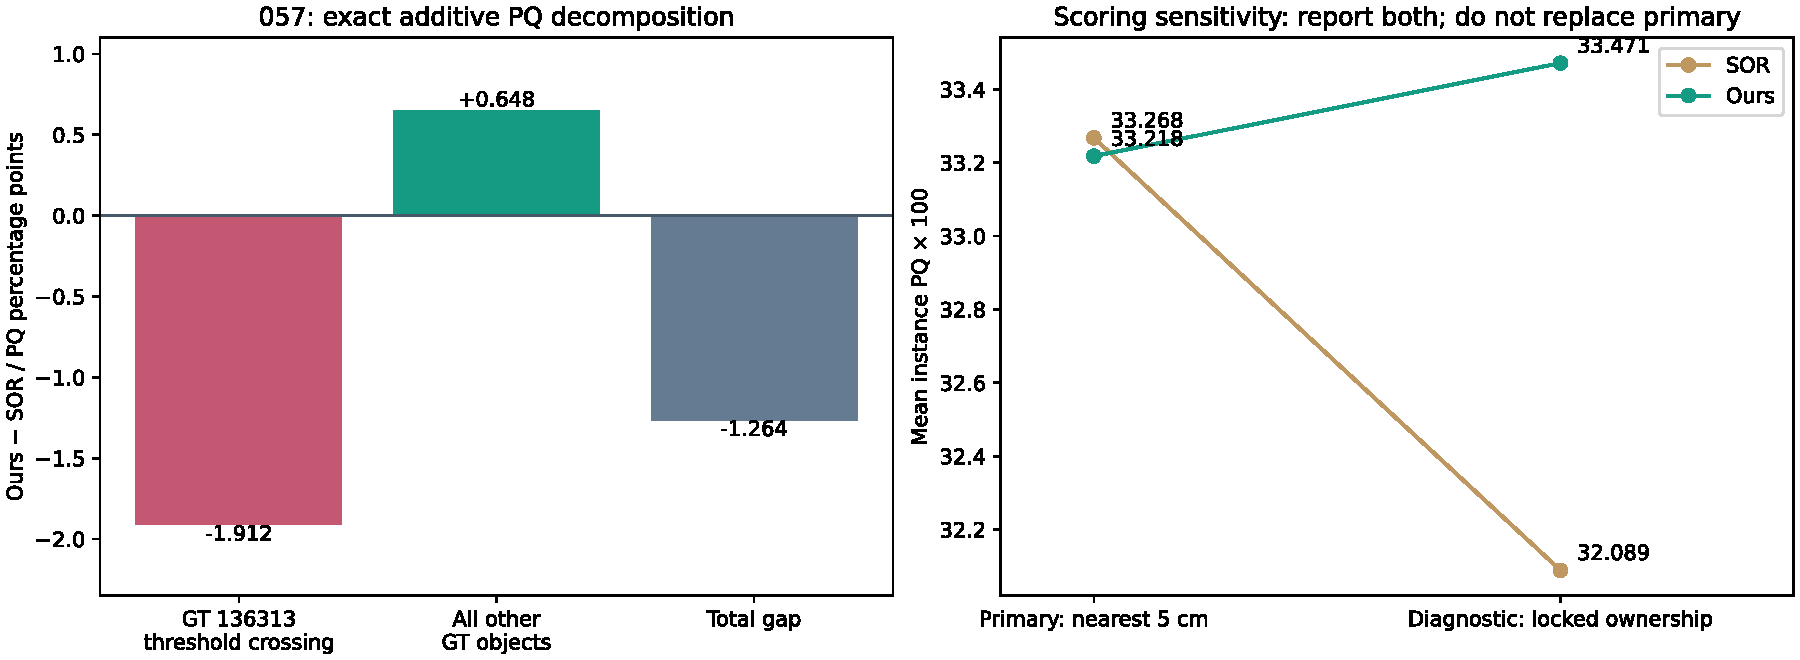
\includegraphics[width=\textwidth]{mechanism_decomposition.pdf}
\captionof{figure}{V1 sequence-057 primary-score deficit relative to SOR: one SOR-only match outweighs gains on the remaining objects. Locking baseline source ownership changes the mean ranking across four scenes. Locked assignment probes reference-label reassignment; it does not replace primary nearest-source evaluation. Embedded ``Ours'' means V1.}
\end{center}
\begin{center}
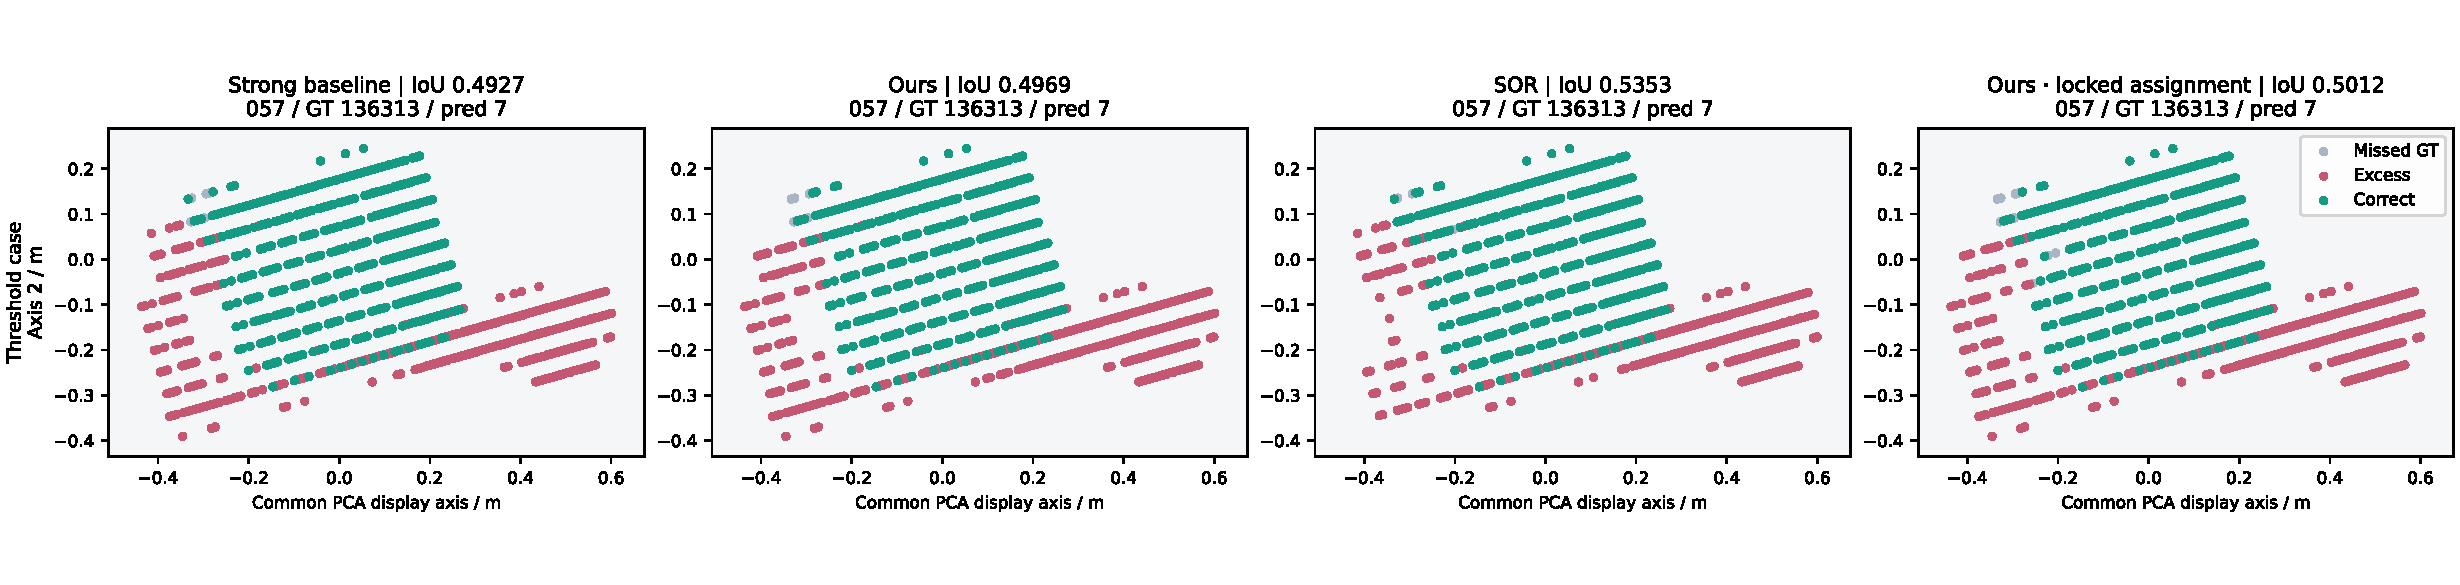
\includegraphics[width=\textwidth]{057_threshold_case.pdf}
\captionof{figure}{Threshold-sensitive GT object 136313 in a shared projection. Correct, excess, and missed reference support are green, red, and gray. The fourth panel locks baseline nearest-source ownership before deletion. All panels show the archived V1 study; ``Ours'' and ``Ours + locked assignment'' are not current-method results.}
\end{center}
The primary IoUs are 0.492718 (strong baseline), 0.496947 (V1), and 0.535340 (SOR). The locked V1 diagnostic is 0.501247. This case illustrates a threshold and ownership interaction, rather than evidence that deleting more points is necessarily better.

\clearpage
\section{Archived Garage Objects and Visual Evidence}\label{app:archived-garage}
\begin{center}
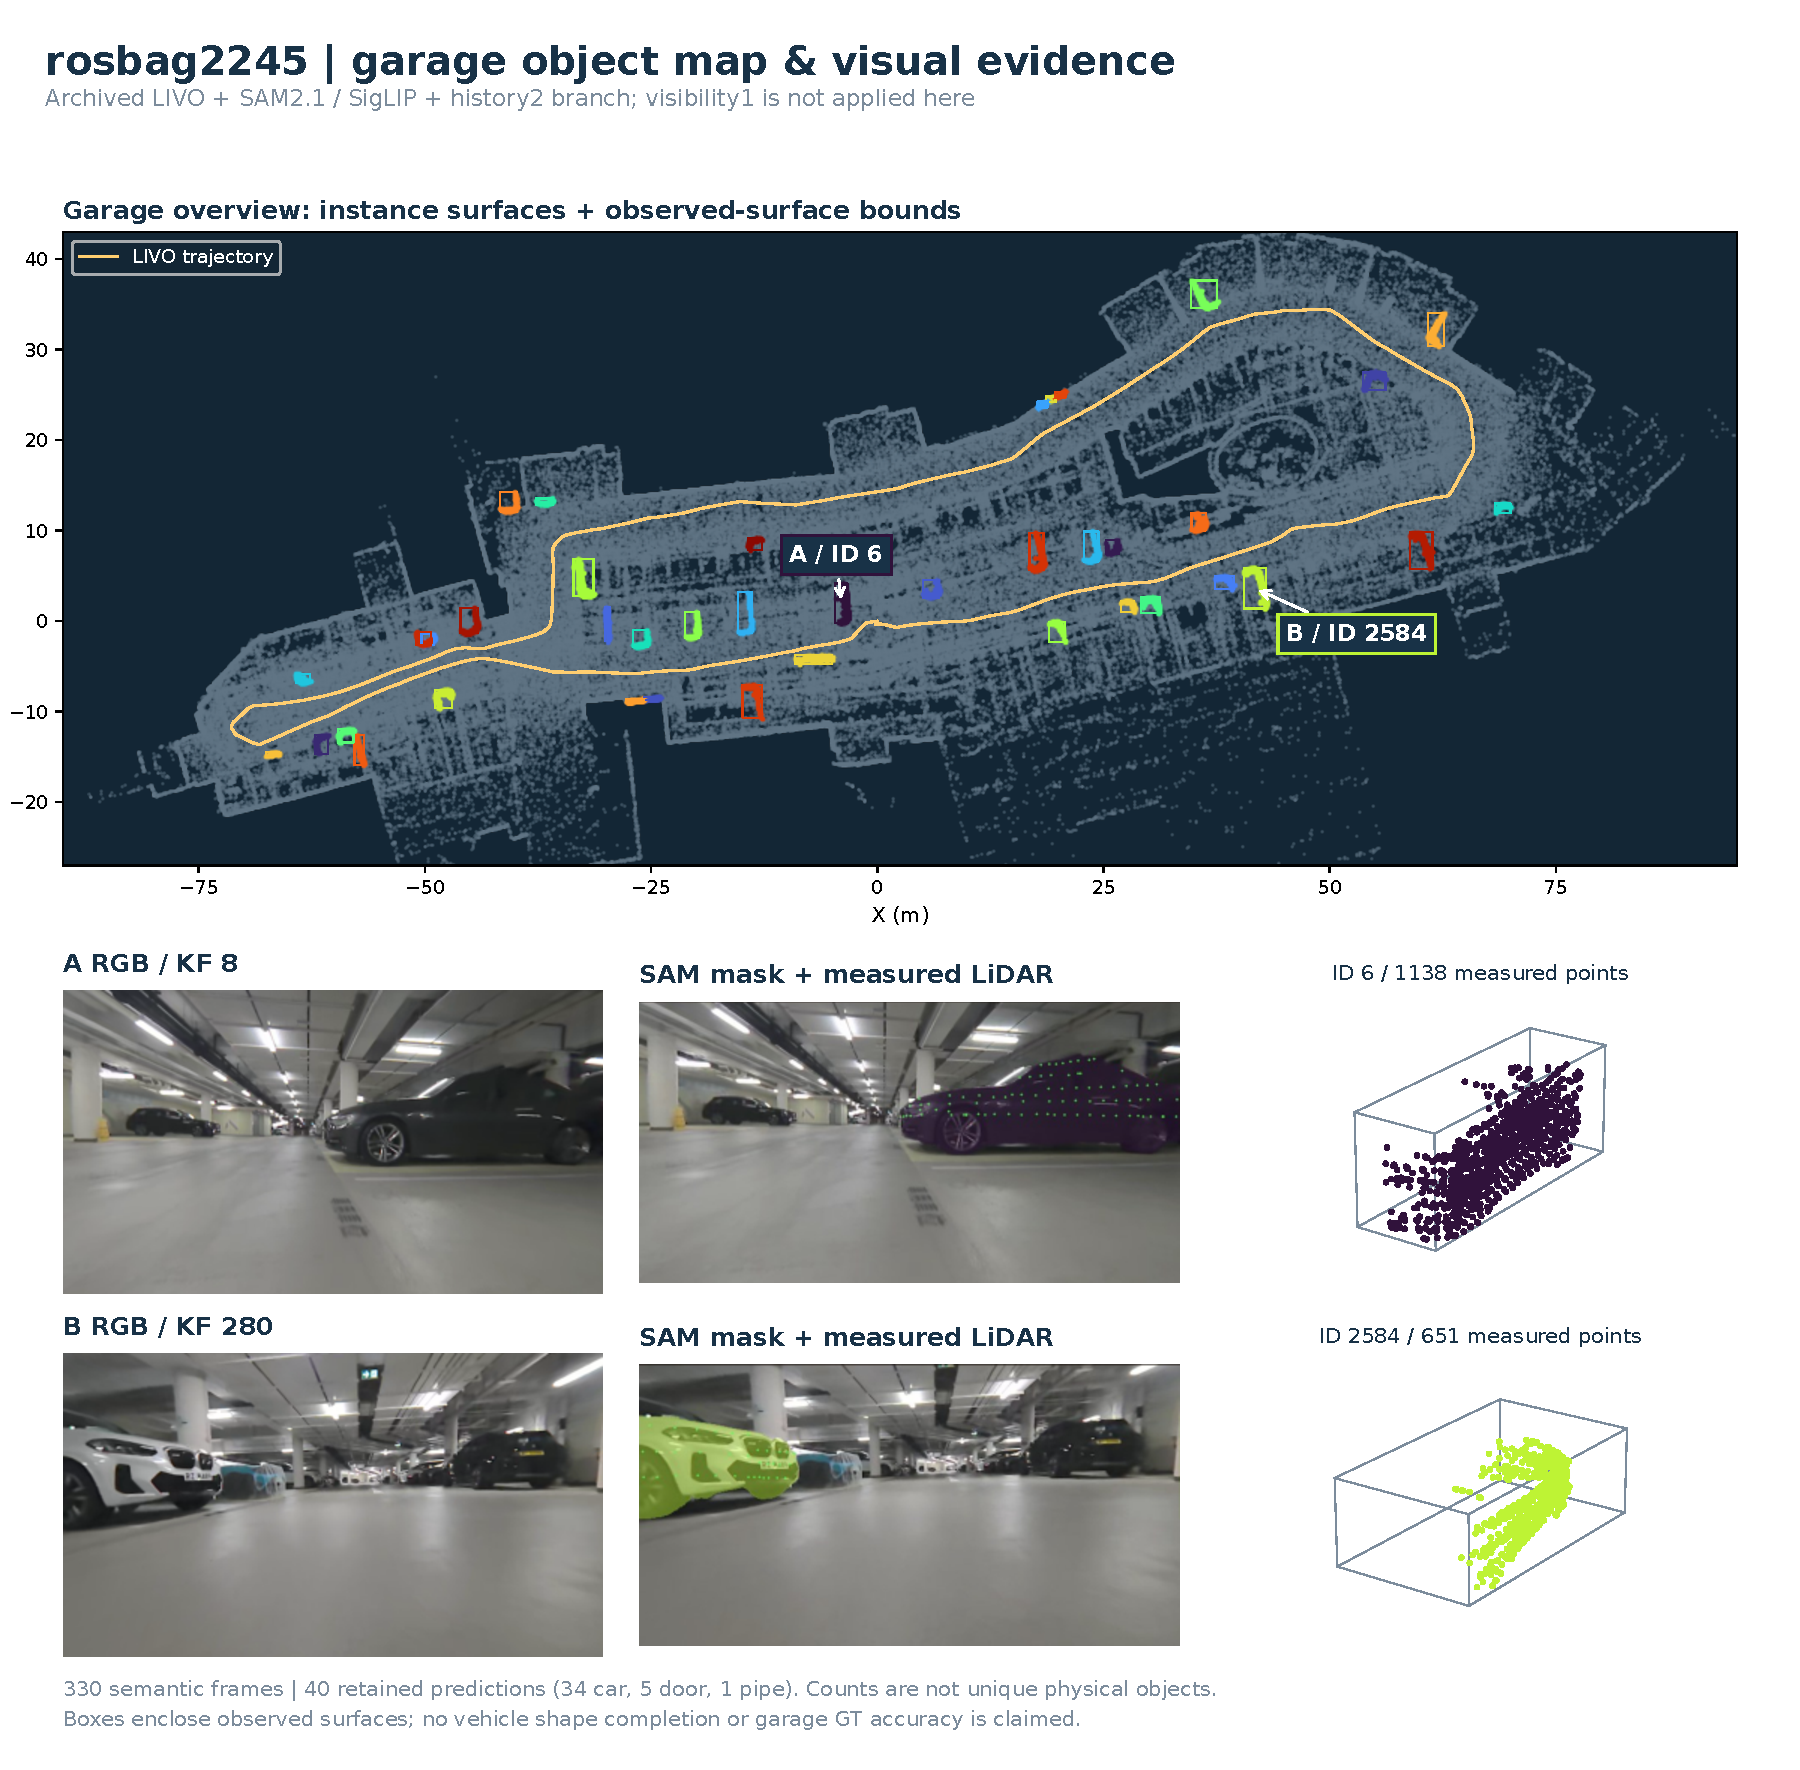
\includegraphics[width=.98\textwidth,height=.76\textheight,keepaspectratio]{garage_real_evidence.pdf}
\captionof{figure}{Archived \texttt{rosbag2245} LIVO + SAM2.1/SigLIP + history2 replay. The map links vehicle records to actual RGB, masks, measured LiDAR support, and accumulated surfaces with boxes. The overview shows all 40 retained predictions with the original crop and context subsampling. Its 330 cached frames produce 34 car, five door, and one pipe records; these are prediction records, not verified unique physical objects. Boxes bound observed surfaces. Neither V1 nor current authorization was applied to this archived map.}
\end{center}
This is the original garage object-evidence view in its own \texttt{omni\_odom} coordinates. It complements the current four-method garage comparison in Appendix~\ref{app:robot}; overlays and IDs are not transferred between these map revisions.

